%%%%%%%%%%%%%%%%%%%%%%%%%%%%%%%%%%%%%%%%%
% Structured General Purpose Assignment
% LaTeX Template
%
% This template has been downloaded from:
% http://www.latextemplates.com
%
% Original author:
% Ted Pavlic (http://www.tedpavlic.com)
%
% Note:
% The \lipsum[#] commands throughout this template generate dummy text
% to fill the template out. These commands should all be removed when 
% writing assignment content.
%
%%%%%%%%%%%%%%%%%%%%%%%%%%%%%%%%%%%%%%%%%

%----------------------------------------------------------------------------------------
%	PACKAGES AND OTHER DOCUMENT CONFIGURATIONS
%----------------------------------------------------------------------------------------

\documentclass{article}

\usepackage{fancyhdr} % Required for custom headers
\usepackage{extramarks} % Required for headers and footers
\usepackage{graphicx} % Required to insert images
\usepackage{enumerate}
\usepackage{amsmath}

% Margins
\topmargin=-0.45in
\evensidemargin=0in
\oddsidemargin=0in
\textwidth=6.5in
\textheight=9.0in
\headsep=0.25in 

\linespread{1.1} % Line spacing

% Set up the header and footer
\pagestyle{fancy}
\lhead{Linear Algebra with Application\\
to Engineering Computation}
\chead{}
\rhead{CME 200/ME300A\\
M. Gerritsen\\
Fall 2013}
\headheight = 40pt

\renewcommand\headrulewidth{0.4pt} % Size of the header rule
\renewcommand\footrulewidth{0.4pt} % Size of the footer rule

\setlength\parindent{0pt} % Removes all indentation from paragraphs

%----------------------------------------------------------------------------------------
%	DOCUMENT STRUCTURE COMMANDS
%	Skip this unless you know what you're doing
%----------------------------------------------------------------------------------------

% Header and footer for when a page split occurs within a problem environment
\newcommand{\enterProblemHeader}[1]{
\nobreak\extramarks{#1}{#1 continued on next page\ldots}\nobreak
\nobreak\extramarks{#1 (continued)}{#1 continued on next page\ldots}\nobreak
}

% Header and footer for when a page split occurs between problem environments
\newcommand{\exitProblemHeader}[1]{
\nobreak\extramarks{#1 (continued)}{#1 continued on next page\ldots}\nobreak
\nobreak\extramarks{#1}{}\nobreak
}

\setcounter{secnumdepth}{0} % Removes default section numbers
\newcounter{homeworkProblemCounter} % Creates a counter to keep track of the number of problems

\newcommand{\homeworkProblemName}{}
\newenvironment{homeworkProblem}[1][Problem \arabic{homeworkProblemCounter}]{ % Makes a new environment called homeworkProblem which takes 1 argument (custom name) but the default is "Problem #"
\stepcounter{homeworkProblemCounter} % Increase counter for number of problems
\renewcommand{\homeworkProblemName}{#1} % Assign \homeworkProblemName the name of the problem
\section{\homeworkProblemName} % Make a section in the document with the custom problem count
\enterProblemHeader{\homeworkProblemName} % Header and footer within the environment
}{
\exitProblemHeader{\homeworkProblemName} % Header and footer after the environment
}
\newcommand\overmat[2]{%
  \makebox[0pt][l]{$\smash{\overbrace{\phantom{%
    \begin{matrix}#2\end{matrix}}}^{\text{$#1$}}}$}#2}

\newcommand{\problemAnswer}[1]{ % Defines the problem answer command with the content as the only argument
\noindent\framebox[\columnwidth][c]{\begin{minipage}{0.98\columnwidth}#1\end{minipage}} % Makes the box around the problem answer and puts the content inside
}

\title{Assignment 1 - Background review}
\date{Issued: \today}
\author{Due: October 2, in class\\
No late assignments accepted}

%----------------------------------------------------------------------------------------

\begin{document}
\maketitle
\thispagestyle{fancy}
\textbf{Important:}
\begin{itemize}
\item Give complete answers: Do not only give mathematical formulae, but explain what you are doing. Conversely, do not leave out critical intermediate steps in mathematical derivations.
\item Write your \textbf{name} as well as your \textbf{Sunet ID} on your assignment. \textbf{Please staple pages together.} Points will be docked otherwise.
\item Questions preceded by * are harder and/or more involved.
\end{itemize}

\begin{homeworkProblem}
Indicate whether the following statements are TRUE or FALSE and motivate your answers clearly. To show a statement false, it is sufficient to give one counter example. To prove a statement true, prove a general proof.
\begin{enumerate}[(a)]
\item If $A^2 + A = I$ then $A^{-1} = I + A $
\item If all diagonal entries of $A$ are zero, then $A$ is singular (not invertible).
\end{enumerate}
\vspace{.5cm}
\problemAnswer{ % Answer
\begin{enumerate}[(a)]
\item True. We have
\begin{equation*}
\begin{aligned}
A^2 + A &= I \\
A(A+I)&=I \\
\end{aligned}
\end{equation*}
Similarly, 
\begin{equation*}
\begin{aligned}
A^2 + A &= I \\
A+A^2&=I \\
(I+A)A&=I\\
\end{aligned}
\end{equation*}
Thus, $$A^{-1} = I+A$$

\item False.  A counterexample is $
\begin{bmatrix}
0 & 1 \\
1 & 0
\end{bmatrix}$,
 which is invertible.
\end{enumerate}
}
\end{homeworkProblem}

\begin{homeworkProblem}
The product of two $n$ by $n$ lower triangular matrices is again lower triangular (all its entries above the main diagonal are zero). Prove it in general and confirm this with a $3$ by $3$ example. 
\newline
\problemAnswer{
Suppose $AB = C$ and $A$ and $B$ are lower-triangular. Recall that, by property of matrix multiplication
$$
c_{ij}=\vec{r_i}^T\vec{b_j}
$$
Consider the $i,j$ element of $C$, only need to show that this element is necessarily $0$ if $i < j$, i.e. above the diagonal, as this is the definition of lower-triangular matrix.
Note that for a lower-triangular matrix, the $i$-th row necessarily has zero after the $i$-th element and the $j$-th column also necessarily has zero until the $j$-th element. Schematically, we have

\begin{equation*}
c_{ij}= \begin{bmatrix}
\overmat{i \hspace{3pt} \text{non-zeros}}{a_1 & a_2 \ldots & a_{i}} & \overmat{n-i \hspace{3pt} \text{zeros}}{0 & 0 \ldots 0 } \\
\end{bmatrix} ^T 
%
\begin{matrix}
 
 \begin{bmatrix}
  0 \\ 0\\ \ \vdots\\0\\b_{j+1}\\b_{j+2}\\ \vdots\\ b_n
  \end{bmatrix}
  \begin{aligned}
  &\left.\begin{matrix}
\cdots\\
\cdots\\
\cdots\\
\cdots\\  

  \end{matrix} \right\} %
  j-1 \text{ zeros}\\

  &\left.\begin{matrix}


  \cdots \\[0.5em]
 \cdots\\ 
\cdots\\
\cdots
  \end{matrix}\right\}
  n-j+1 \text { nonzeros}\\
 \end{aligned}
 \end{matrix} = \quad 0
 \end{equation*}
because $j-1 \geq i$ and $n-j+1 \leq n-i.$
}
\end{homeworkProblem}

\begin{homeworkProblem}
If $A = A^T$ and $B = B^T$ , which of these matrices are certainly symmetric? A counter-example would be sufficient to prove that the statement is false, but to prove it is true
\begin{enumerate}[(a)]
\item $A^2 - B^2$
\item $(A + B)(A - B)$
\item $ABA$
\item $ABAB$
\end{enumerate}
\problemAnswer{ % Answer
\begin{enumerate}[(a)]
\item True
\begin{align}
(A^2 - B^2)^T &= (AA)^T - (BB)^T \\
&= A^TA^T - B^TB^T \\
&= A^2 - B^2
\end{align}
\item False, 
\begin{align}
(A+B)(A-B) &= A^2 +BA - AB - B^2
\end{align}
\begin{align}
[(A+B)(A-B)]^T&=[A^2 +BA - AB - B^2]^T \\
 &= (A^2)^T +(BA)^T - (AB)^T - (B^2)^T\\
 &=(A^T)^2+A^TB^T-B^TA^T-B^TB^T\\
 &=A^2+AB-BA-B^2\\ 
\end{align}
But$$AB \neq BA \quad\text{in general, (although they can be equivalent, in which case we say $A$ and $B$ {\it commute})}$$

\item True
\begin{align}
(ABA)^T = A^TB^TA^T = ABA
\end{align}
\item False
\begin{align}
(ABAB)^T = B^TA^TB^TA^T = BABA \neq ABAB \text{ because matrices do not commute in general}
\end{align}
\end{enumerate}
}
\end{homeworkProblem}

\begin{homeworkProblem}
A {\it skew-symmetric} matrix is a matrix that satisfies $A^T=-A$.  Prove that if $A$ is $n\times n$ and skew-symmetric, than for any $\vec{x}$, we must have that $\vec{x}^TA\vec{x} = 0$.
\newline

\problemAnswer{
Since $A$ is $n\times n$, $\vec{x}$ must be $n\times 1$, which is consistent with our view of all vectors as {\it column} vectors.  Then the product $A\vec{x}$ must also be a column vector of the same size as $\vec{x}$.  Call this column vector $\vec{y}$.  Then
$$\vec{x}^TA\vec{x}=\vec{x}^T(A\vec{x})=\vec{x}^T\vec{y}$$

But we recognize $\vec{x}^T\vec{y}$ as a scalar product, and so $\vec{x}^TA\vec{x}$ is a scalar quantity.  Now, a nice property of scalars is that they equal their own transpose, so for any $\vec{x}$, 
we have that 
$$\vec{x}^TA\vec{x} = (\vec{x}^TA\vec{x})^T$$
By skew symmetry of $A$, we then have that 
$$\vec{x}^TA\vec{x}=(\vec{x}^TA\vec{x})^T=\vec{x}^TA^T\vec{x}=\vec{x}^T(-A)\vec{x}=-(\vec{x}^TA\vec{x})$$
The only scalar that satisfies this equation is 0.
}
\end{homeworkProblem}


\begin{homeworkProblem}
Suppose $A$ is an $n\times n$ invertible matrix, and you exchange its first two rows to create a new matrix $B$.  Is the new matrix $B$ necessarily invertible?  If so, how could you find $B^{-1}$ from $A^{-1}$?  If not, why not?
\newline

\problemAnswer{
As we know, swapping rows does not change the represented system of equations.  Swapping the first and second row is equivalent to premultiplying $A$ by an elementary matrix $E=E_{12}$ to get $B$, where $E_{12}$ is the identity with its first two rows swapped, i.e.,
$$E_{12}=\begin{pmatrix}0 & 1 & 0 & \cdots & 0\\
1 & 0 & 0 & \dots & 0\\
0 & 0 & 1 & \ddots & 0\\
\vdots & \vdots & \ddots & \ddots & 0\\
0 & 0 & \cdots & 0 & 1
\end{pmatrix}$$.  

So we write $$B=E_{12}A,$$ which implies $$B^{-1} = (E_{12}A)^{-1} = A^{-1}E_{12}^{-1}$$  Now, we know that $E_{12}$ is invertible, because multiplying $E_{12}$ by itself returns the identity matrix. So, $(E_{12})^{-1}=E_{12}.$  But now
$$B^{-1}=A^{-1}E_{12}^{-1}=A^{-1}E_{12}.$$

Since we are {\it post}-multiplying $A^{-1}$ by $E_{12}$, we are swapping the first two {\it columns} of $A^{-1}$ to get $B^{-1}$.

}
\end{homeworkProblem}


\begin{homeworkProblem}
Let $A$ be an invertible $n$-by-$n$ matrix.  Prove that $A^m$ is also invertible and that $$\left(A^m\right)^{-1} = \left(A^{-1}\right)^m$$ for $m= 1, 2, 3,  \ldots$ 
\newline

\problemAnswer{
We want to show that for any integer value of $m$, the inverse of $A^m$ is the inverse of $A$ raised to the $m$-th power.  In other words, we want to show that $$A^m(A^{-1})^m= (A^{-1})^mA^m=I$$  We prove this by induction on $m$.  \\

(i) First, we look at the base case, i.e., the case $m=1$:\\
$$(A^1)^{-1} = A^{-1} = (A^{-1})^1$$.  

(ii) Next, we {\it assume} that the result holds for some arbitrary value $m=k$:
$$\text{Assume } (A^k)^{-1}=(A^{-1})^k$$

(iii) Now, using steps i) and ii), we {\it show} the result holds for $m=k+1$:
$$(A^{-1})^{k+1}A^{k+1} = A^{-1}(A^{-1})^kA^kA=A^{-1}(A^k)^{-1}A^kA=A^{-1}IA=I$$
and
$$A^{k+1}(A^{-1})^{k+1} = AA^k(A^{-1})^kA^{-1} = AA^k(A^k)^{-1}A^{-1}=AIA^{-1}=I$$
\newline
where we have used the result in part (ii).  Thus, the general result follows by the induction principle. 

}
\end{homeworkProblem}


\begin{homeworkProblem}[Problem \arabic{homeworkProblemCounter}]
Let $A$ be a $2\times 2$ matrix $\left( \begin{array}{cc}
a_{11} & a_{12} \\
a_{21} & a_{22} \end{array} \right)$ with $a_{11} \neq 0$ and let $\alpha = a_{21}/a_{11}$.  Show that $A$ can be factored into a product of the form
\[ \left( \begin{array}{cc}
1 & 0 \\
\alpha & 1 \end{array} \right) 
\left( \begin{array}{cc}
a_ {11} & a_{12}\\
0 & b  \end{array} \right)\]

What is the value of $b$?
\newline

\problemAnswer{
If $\alpha = a_{21}/a_{11}$, then multiplying the matrices in the factorization gives

\[ \left( \begin{array}{cc}
1 & 0 \\
\alpha & 1 \end{array} \right) 
\left( \begin{array}{cc}
a_ {11} & a_{12}\\
0 & b  \end{array} \right)   = 
%%%%%%%%%%%%%%%
 \left( \begin{array}{cc}
a_{11} & a_{12} \\
{\alpha}a_{11} & {\alpha}a_{12}+b \end{array} \right) =
%%%%%%%%%%%%%%%
 \left( \begin{array}{cc}
a_{11} & a_{12} \\
a_{21} & {\alpha}a_{12}+b \end{array} \right) .
\]
\newline
This product will equal the original $A$ provided $${\alpha}a_{12} + b = a_{22}$$  Thus, we must have that $$b = a_{22}-{\alpha}a_{12}=a_{22}-\frac{a_{21}a_{12}}{a_{11}}$$

}
\end{homeworkProblem}

\begin{homeworkProblem}[Problem \arabic{homeworkProblemCounter}*]
\begin{enumerate}[(a)]
\item Show that if the $n\times n$ matrices $A$ and $B$ are invertible, and if the matrix $A+B$ is also invertible, then the matrix $B^{-1} + A^{-1}$ is also invertible. 
\item Assume that $C$ is a skew-symmetric matrix and that $D$ is a matrix defined as $$D=(I+C)(I-C)^{-1}$$  Prove that $D^TD=DD^T=I.$
\end{enumerate}
\problemAnswer{
\begin{enumerate}[(a)]

\item We must find a matrix, call it $M$, such that $$(A^{-1}+B^{-1})M=I$$
 Using the fact that $A, B$ and $A+B$ are invertible, we will do some algebraic manipulations to simplify to something we are given. We write
\begin{equation*}
   \begin{aligned}
    I 	&=  (A^{-1}+B^{-1})M\\
       	&= (A^{-1}+IB^{-1})M \\
       	&= (A^{-1}+A^{-1}AB^{-1})M \\
       	&= A^{-1}(I+AB^{-1})M\\
       	&=A^{-1}(BB^{-1}+AB^{-1})M\\
	&=A^{-1}(B+A)B^{-1}M
     \end{aligned}
\end{equation*}
From the last equation, we see that $$\left(A^{-1}(B+A)B^{-1}\right)M=I$$
Therefore, $M=\left(A^{-1}(A+B)B^{-1}\right)^{-1}=B(A+B)^{-1}A$

Now we verify that multiplying $M$ on the right by the original matrix also gives the identity:
\begin{equation*}
   \begin{aligned}
	M(A^{-1}+B^{-1}) &= B(A+B)^{-1}A(A^{-1}+B^{-1}) \\
       	&=B(A+B)^{-1}(AA^{-1}+AB^{-1})\\
&=B(A+B)^{-1}(I+AB^{-1})\\
       	&=B(A+B)^{-1}(BB^{-1}+AB^{-1})\\
	&= B(A+B)^{-1}(B+A)B^{-1} \\
       	&= BB^{-1} \\
       	&= I
     \end{aligned}
\end{equation*}
Therefore, we have that, indeed $(B^{-1} + A^{-1})^{-1}=B(A+B)^{-1}A$

\item  The trick here is to observe that $(I+C)$ and $(I-C)$ commute, that is, $$(I+C)(I-C)=(I-C)(I+C)$$  Then
\begin{equation*}
   \begin{aligned}
    D^TD 	&=  [(I+C)(I-C)^{-1}]^T(I+C)(I-C)^{-1}\\
       	&= [(I-C)^T]^{-1}(I+C)^T(I+C)(I-C)^{-1} \\
       	&= (I-C^T)^{-1}(I+C^T)(I+C)(I-C)^{-1} \\
       	&= (I+C)^{-1}(I-C)(I+C)(I-C)^{-1} \\
	&=(I+C)^{-1}(I+C)(I-C)(I-C)^{-1}\\
	&=I
     \end{aligned}
\end{equation*}
\end{enumerate}
Going from the first line to the second line, we have used properties of transposes as well as the interchanging of transposition and inversion. Going from the second line to the third line, we have used the property for the transpose of a sum of matrices. Going from the third line to the fourth line, we've used the fact that $C$ is skew-symmetric. Going from the fourth line to the fifth line, we're using the fact that $(I+C)$ and $(I-C)$ commute. 
}
\problemAnswer{
To show $DD^T=I$ we can follow similarly:
\begin{equation*}
   \begin{aligned}
    DD^T 	&=  (I+C)(I-C)^{-1}[(I+C)(I-C)^{-1}]^T\\
       	&= (I+C)(I-C)^{-1}[(I-C)^T)^{-1}(I+C)^T] \\
       	&= (I+C)(I-C)^{-1}(I-C^T)^{-1}(I+C^T) \\
       	&= (I+C)(I-C)^{-1}(I+C)^{-1}(I-C) \\
	&=(I+C)[(I+C)(I-C)]^{-1}(I-C)\\
	&=(I+C)[(I-C)(I+C)]^{-1}(I-C)\\
	&=(I+C)(I+C)^{-1}(I-C)^{-1}(I-C)\\
	&=I
     \end{aligned}
\end{equation*}
where again we have used the fact that $(I-C)$ and $(I+C)$ commute.
}


\end{homeworkProblem}

\begin{homeworkProblem}[Problem \arabic{homeworkProblemCounter}*]
Given an $n \times n$ matrix $A$ with column vectors $\vec{a_1},\vec{a_2},\ldots,\vec{a_n},$ construct a matrix $B$ such that the matrix $AB$ has the columns $\vec{u_1},\vec{u_2},\ldots,\vec{u_n}$ with the following properties:
\begin{enumerate}[(i)]
\item $\vec{u_i} = \vec{a_i}, \quad i \neq j$
\item $\vec{u_j} = \sum_{k=1}^j\alpha_k\vec{a_k}$,
\end{enumerate}
where $j$ is a {\it fixed} integer such that $1\leq j \leq n$.
\newline

\problemAnswer{ Writing out the matrices in terms of their columns, we have
$$A = \left[\vec{a_1},\vec{a_2},\ldots,\vec{a_n}\right]$$
$$AB = \left[\vec{u_1},\vec{u_2},\ldots,\vec{u_n}\right]$$
$$B = \left[\vec{b_1},\vec{b_2},\ldots,\vec{b_j},\ldots,\vec{b_n}\right]$$
Note that $j$ is a fixed integer indexing a column $\vec{b_j}$ between 1 and $n$ in the matrix  $B$. Aside from $\vec{u_j}$, the columns of $AB$ and $A$ are the same.
Thus, $B$ looks like the identity matrix {\it except} for column $\vec{b_j}$.  Writing out the $j$-th column of the matrix $AB$ in terms of the {\it columns of A}, we have 
$$\vec{(AB)_j} = \vec{u_j} = b_{1j}\vec{a_1} + b_{2j}\vec{a_2} +\dots+b_{jj}\vec{a_j}+\dots+b_{nj}\vec{a_n}$$  Thus, we see that
$$\alpha_k = b_{kj} \text{ for all } k \text{ such that } 1\leq k \leq j.$$
Here is a schematic of $B$:
\begin{center}
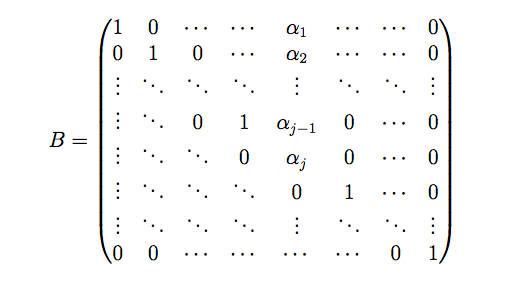
\includegraphics[width=4in]{matrixB.jpg}
\end{center}
}
\end{homeworkProblem}

\end{document}
